\chapter{Background}
\label{chapter: background}

\section{Edge Computing}

Edge computing is a nascent computing paradigm that has gain significant
tractions over the past few years. It aims to address the problem of
over-centralization in which. Gabriel applications offload computation to a
cloudlet, a small data-center at the edge of the
internet~\cite{satyanarayanan2009case}. The high bandwidth and low latency
offered by cloudlets~\cite{ha2013impact}~\cite{hu2016quantifying} lay the
foundation of wearable cognitive assistance~\cite{ha2014towards}. Previous
research has worked on VM synthesis~\cite{ha2013just} to enable rapid
provisioning of applications onto a cloudlet. In addition, user mobility is
supported through VM handoff~\cite{ha2017you}, which migrates user states from
one cloudlet to another. These pioneer work into cloudlet together with
decade-long research into computational
offload~\cite{cuervo2010maui}~\cite{gordon2012comet}~\cite{flinn2012cyber}
provides the infrastructure support that makes wearable cognitive assistance
applications feasible. Previous measurement of edge computing's impact on mobile
applications tested compute-intensive and latency-sensitive applications when
network utilization is low~\cite{chen2017empirical}. This work relaxes such
assumption and focuses on supporting more users when the resource utilization is
high.


\section{Gabriel Platform}

\begin{figure}
\centering
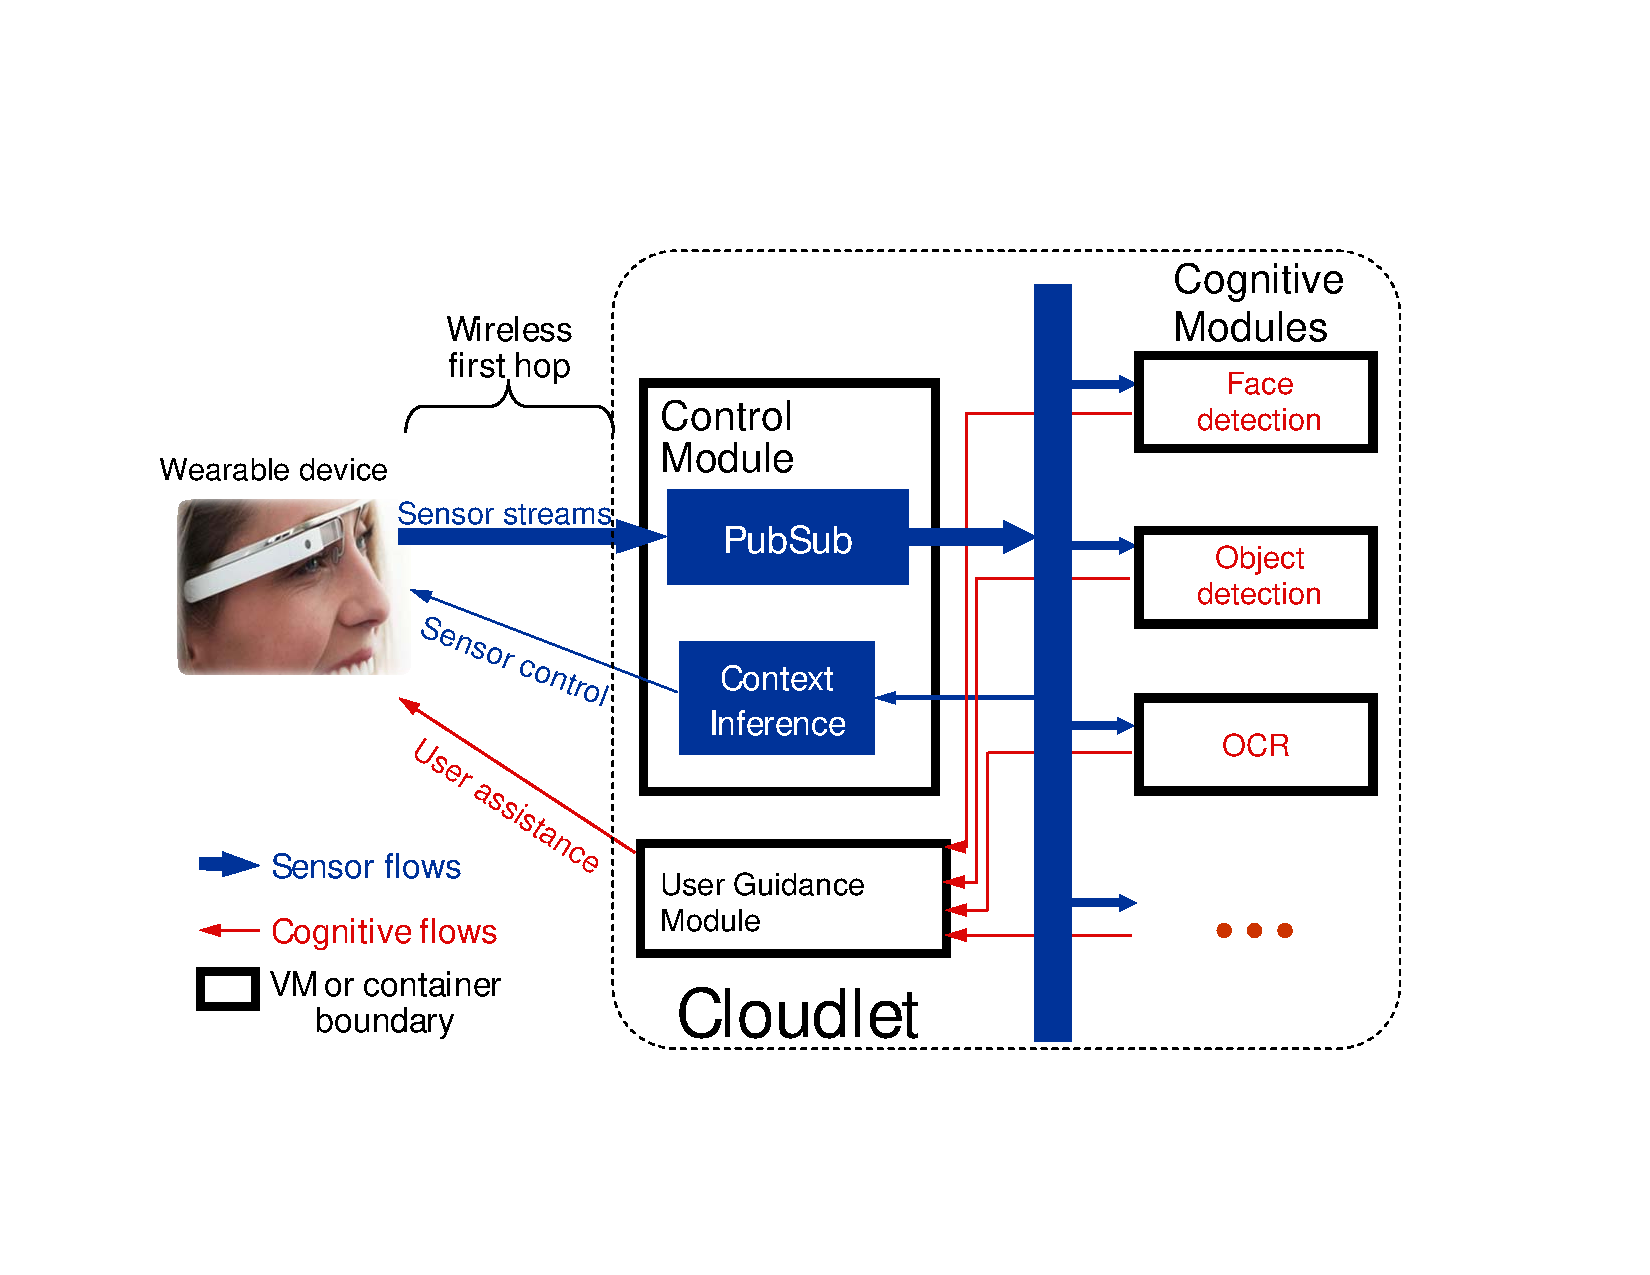
\includegraphics[width=0.8\linewidth]{FIGS/fig-backend-structure-simple-crop.pdf}
\begin{captiontext}
{\rm (Source: Chen et al~\cite{chen2017empirical})}
\end{captiontext}
\caption{\small Gabriel Platform}
\label{fig:gabriel}
\end{figure}

The Gabriel platform~\cite{ha2014towards,chen2017empirical}, shown in
Figure~\ref{fig:gabriel}, is the first implementation of WCA and provides an
application framework to simplify development. The Gabriel front-end on a
wearable device performs preprocessing of sensor data (e.g., compression and
encoding), which it streams over a wireless network to a cloudlet.  The Gabriel
back-end on the cloudlet has a modular structure. The {\em control module} is
the focal point for all interactions with the wearable device.  A
publish-subscribe (PubSub) mechanism decodes and distributes the incoming sensor
streams to multiple {\em cognitive modules} (e.g., task-specific computer vision
algorithms) for concurrent processing. Cognitive module outputs are integrated
by a task-specific {\em user guidance module} that performs higher-level
cognitive processing such as inferring task state, detecting errors, and
generating guidance in one or more modalities (e.g., audio, video, text, etc.).

The original Gabriel platform was built with a single user in mind,
and did not have mechanisms to share cloudlet resources in a
controlled manner.  It did, however, have a token-based transmission
mechanism.  This limited a client to only a small number of
outstanding operations, thereby offering a simple form of rate
adaptation to processing or network bottlenecks.  We have retained
this token mechanism in our system, described in the rest of this paper.
In addition, we have extended Gabriel with new mechanisms to handle
multitenancy, perform resource allocation, and support
application-aware adaptation.  We refer to the two versions of the
platform as ``Original Gabriel'' and ``Scalable Gabriel.''

\section{Example Gabriel Applications}

Many applications have been built on top of the Gabriel platform.  Recent
papers~\cite{chen2017empirical}~\cite{chen2018application} describe these applications,
along with detailed analysis of their end-to-end latency. For example, the LEGO
application guides a user to construct a Lego model, step by step, continuously
monitoring the task with computer vision, and providing instructions when it has
detected that the user has completed a step. POOL assists a user in aiming a
pool cue stick. PING PONG suggests hitting a ball to the left or right to win a
rally in table tennis. FACE recognizes a face that has appeared in a scene,
searches the user's personal database, and whispers the person's name. IKEA
helps a user to assemble an IKEA lamp step by step.

These applications run on multiple wearable devices such as Google
Glass, Microsoft HoloLens, Vuzix Glass, and ODG R7. At a high level, 
the cloudlet workflows of these applications are similar, and consist of
two major phases.  The first phase uses computer vision
to extract a symbolic, idealized representation of the state of the
task, accounting for real-world variations in lighting, viewpoint,
etc.  The second phase operates on the symbolic representation,
implements the logic of the task at hand, and occasionally generates
guidance for the user.  In most WCA applications, the first phase is
far more compute intensive than the second phase.

